\chapter{RVfpga}
\label{chapter:rvfpga}
\section{Baseline SoC: RVfpgaNexys}
In section \ref{section:RISCV}, after analyzing several different RISC-V based SoCs, the SweRVolf SoC was chosen as the baseline SoC for this thesis. RVfpgaNexys is an extended version of SweRVolf targeted to the Nexys A7 board. The extended SweRVolf, or SweRVolfX, adds 4 peripherals to SweRVolf: a GPIO interface for the board's LEDs and switches, a PTC, an additional SPI, and a controller for the 8 digit 7-Segment Displays.

\begin{figure}[h]
    \centering
    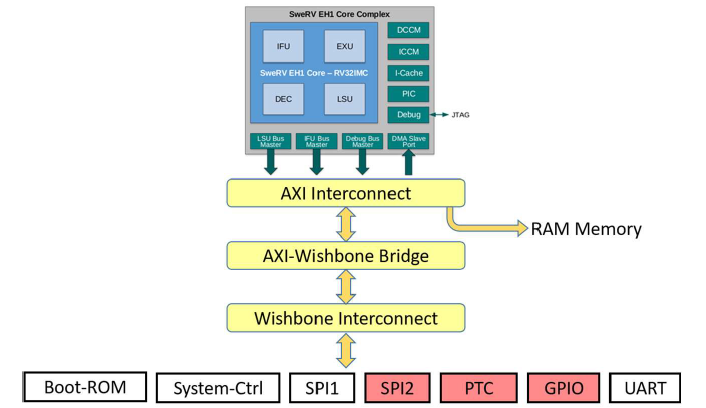
\includegraphics[scale=0.7]{Figures/SweRVolfX.png}
    \caption{SweRVolfX block diagram from Imagination Technologies}
    \label{fig:SweRVolfX}
\end{figure}

Figure \ref{fig:SweRVolfX} shows the block diagram of the SweRVolfX SoC. The SoC utilizes the SweRV EH1 Core Complex from Western DIgital with a 32-bit (RV32ICM) core. The SweRVolf SoC includes a Boot ROM, UART, a System Controller and an SPI controller. The peripherals use a Wishbone bus, however the SweRV EH1 Core uses AXI, so the SoC also includes a AXI to Wishbone bridge. The RAM memory is connected to the processor through the AXI interconnect.

\begin{figure}[H]
    \centering
    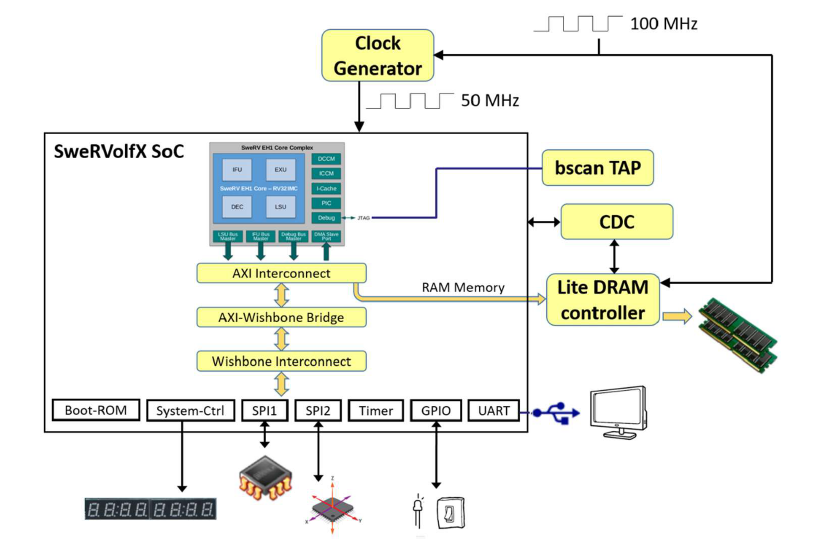
\includegraphics[scale=0.5]{Figures/RVfpgaNexys.png}
    \caption{RVfpgaNexys block diagram from Imagination Technologies}
    \label{fig:RVfpgaNexys}
\end{figure}

Figure \ref{fig:RVfpgaNexys} has a block diagram that shows how the SweRVolfX SoC and the Nexys A7 board interact with each other.

TODO Recursos utilizados pela SoC
TODO Benchmarks corridos

\section{AXI Interconnect}
TODO Explicar AXI Interconnect
TODO O que é preciso adicionar?
TODO Primeiro tentei modificar o interconnect que já lá estava. Porque não funcionou?
TODO Depois tentei utilizar uma opção open source para manter a SoC completamente simulável e open source. Porque é que não deu?
TODO Finalmente utilizei o AXI interconnect da xilinx. Porque foi a melhor opção?
TODO Quais são os ports que lá estão e para que servem?
TODO Recursos utilizados pela SoC e comparar com a versão anterior
TODO Benchmarks corridos e comparar com a versão anterior

\section{Hardware Accelerator}
TODO Explicar acelerador
TODO Qual é o funcionamento básico do acelerador?
TODO Como o desenhei no HLS? Quais foram os recursos utilizados para o acelerador?
TODO Como é que a SoC interaje com o acelerador?
TODO Recursos utilizados pela SoC e comparar com a versão anterior
TODO Benchmarks corridos e comparar com a versão anterior